
%(BEGIN_QUESTION)
% Copyright 2006, Tony R. Kuphaldt, released under the Creative Commons Attribution License (v 1.0)
% This means you may do almost anything with this work of mine, so long as you give me proper credit

Differential pressure transmitters are very common in the process industries.  Besides being used to measure pressure (both differential and gauge), they may also be used to infer fluid level, fluid flow, and fluid density.  A standard manifold called a {\it three-valve manifold} is often used to connect a differential pressure transmitter to the process.  These manifolds consist of two block valves (to isolate the ``high'' and ``low'' transmitter ports from the process) and one ``equalizing'' valve (to connect both ports together to ensure zero differential pressure).

Three-valve manifolds are usually found as single units: a billet of metal with valves and ports machined into it, ready to bolt directly to a transmitter.  However, you can build your own three-valve manifold using three individual valves, two tee fittings, and whatever other fittings are necessary to connect to the transmitter.

\vskip 10pt

Suppose we encounter a differential pressure transmitter used to measure pressure drop across a heat exchanger.  The typical pressure on the upstream side of this heat exchanger is 1000 PSI, while the typical pressure on the downstream side of this exchanger is 970 PSI.  The transmitter connects to this heat exchanger via a three-valve manifold.  A single ``bleed'' valve installed on the transmitter's low-pressure side is used to vent pressure to atmosphere prior to removal of the transmitter from the manifold:

$$\includegraphics[width=15.5cm]{i00211x01.eps}$$

The common procedure for operating a 3-valve manifold to take a transmitter out of service is to first close the high-side block valve, then open the equalizing valve, then close the low-side block valve.  Once these manifold valves have been thus arranged to isolate the transmitter from the process and equalize differential pressure inside the transmitter, the bleed valve may be carefully opened to release stored pressure to atmosphere.

Determine how much fluid pressure will be on each side of the transmitter through every step of this procedure:

% No blank lines allowed between lines of an \halign structure!
% I use comments (%) instead, so that TeX doesn't choke.

$$\vbox{\offinterlineskip
\halign{\strut
\vrule \quad\hfil # \ \hfil & 
\vrule \quad\hfil # \ \hfil & 
\vrule \quad\hfil # \ \hfil & 
\vrule \quad\hfil # \ \hfil \vrule \cr
\noalign{\hrule}
%
% First row
Step & High-side pressure & Low-side pressure & Differential pressure \cr
%
\noalign{\hrule}
%
% Another row
Transmitter in service & 1000 PSI & 970 PSI & 30 PSID \cr
%
\noalign{\hrule}
%
% Another row
Close high-side block valve &  &  &  \cr
%
\noalign{\hrule}
%
% Another row
Open equalizing valve &  &  &  \cr
%
\noalign{\hrule}
%
% Another row
Close low-side block valve &  &  &  \cr
%
\noalign{\hrule}
%
% Another row
Open bleed valve &  &  &  \cr
%
\noalign{\hrule}
} % End of \halign 
}$$ % End of \vbox

Now, suppose someone else (at a later date) were to remove this transmitter from service using the three-valve manifold, but following a different order of steps: closing the low-side block valve first, then equalizing, then blocking the high side.

Determine how much fluid pressure will be on each side of the transmitter through every step of this (alternative) procedure:

% No blank lines allowed between lines of an \halign structure!
% I use comments (%) instead, so that TeX doesn't choke.

$$\vbox{\offinterlineskip
\halign{\strut
\vrule \quad\hfil # \ \hfil & 
\vrule \quad\hfil # \ \hfil & 
\vrule \quad\hfil # \ \hfil & 
\vrule \quad\hfil # \ \hfil \vrule \cr
\noalign{\hrule}
%
% First row
Step & High-side pressure & Low-side pressure & Differential pressure \cr
%
\noalign{\hrule}
%
% Another row
Transmitter in service & 1000 PSI & 970 PSI & 30 PSID \cr
%
\noalign{\hrule}
%
% Another row
Close low-side block valve &  &  &  \cr
%
\noalign{\hrule}
%
% Another row
Open equalizing valve &  &  &  \cr
%
\noalign{\hrule}
%
% Another row
Close high-side block valve &  &  &  \cr
%
\noalign{\hrule}
%
% Another row
Open bleed valve &  &  &  \cr
%
\noalign{\hrule}
} % End of \halign 
}$$ % End of \vbox

Based on the pressures seen by the transmitter in both procedures, would you recommend one procedure over the other?  If so, why?

\vskip 20pt \vbox{\hrule \hbox{\strut \vrule{} {\bf Suggestions for Socratic discussion} \vrule} \hrule}

\begin{itemize}
\item{} A powerful problem-solving technique is performing a {\it thought experiment} where you mentally simulate the response of a system to some imagined set of conditions.  Explain how this particular thought experiment is helpful in determining which is the safest procedure for operating a three-valve transmitter manifold.
\end{itemize}

\underbar{file i00211}
%(END_QUESTION)





%(BEGIN_ANSWER)

%(END_ANSWER)





%(BEGIN_NOTES)

Following the procedure ``HEL'' (High-side, Equalizer, then Low-side):

% No blank lines allowed between lines of an \halign structure!
% I use comments (%) instead, so that TeX doesn't choke.

$$\vbox{\offinterlineskip
\halign{\strut
\vrule \quad\hfil # \ \hfil & 
\vrule \quad\hfil # \ \hfil & 
\vrule \quad\hfil # \ \hfil & 
\vrule \quad\hfil # \ \hfil \vrule \cr
\noalign{\hrule}
%
% First row
Step & High-side pressure & Low-side pressure & Differential pressure \cr
%
\noalign{\hrule}
%
% Another row
Transmitter in service & 1000 PSI & 970 PSI & 30 PSID \cr
%
\noalign{\hrule}
%
% Another row
Close high-side block valve & 1000 PSI & 970 PSI & 30 PSID \cr
%
\noalign{\hrule}
%
% Another row
Open equalizing valve & 970 PSI & 970 PSI & 0 PSID \cr
%
\noalign{\hrule}
%
% Another row
Close low-side block valve & 970 PSI & 970 PSI & 0 PSID \cr
%
\noalign{\hrule}
%
% Another row
Open bleed valve & 0 PSI & 0 PSI & 0 PSID \cr
%
\noalign{\hrule}
} % End of \halign 
}$$ % End of \vbox

\vskip 10pt

Following the procedure ``LEH'' (Low-side, Equalizer, then High-side):

% No blank lines allowed between lines of an \halign structure!
% I use comments (%) instead, so that TeX doesn't choke.

$$\vbox{\offinterlineskip
\halign{\strut
\vrule \quad\hfil # \ \hfil & 
\vrule \quad\hfil # \ \hfil & 
\vrule \quad\hfil # \ \hfil & 
\vrule \quad\hfil # \ \hfil \vrule \cr
\noalign{\hrule}
%
% First row
Step & High-side pressure & Low-side pressure & Differential pressure \cr
%
\noalign{\hrule}
%
% Another row
Transmitter in service & 1000 PSI & 970 PSI & 30 PSID \cr
%
\noalign{\hrule}
%
% Another row
Close low-side block valve & 1000 PSI & 970 PSI & 30 PSID \cr
%
\noalign{\hrule}
%
% Another row
Open equalizing valve & 1000 PSI & 1000 PSI & 0 PSID \cr
%
\noalign{\hrule}
%
% Another row
Close high-side block valve & 1000 PSI & 1000 PSI & 0 PSID \cr
%
\noalign{\hrule}
%
% Another row
Open bleed valve & 0 PSI & 0 PSI & 0 PSID \cr
%
\noalign{\hrule}
} % End of \halign 
}$$ % End of \vbox

\vskip 10pt

The HEL procedure results in less pressure being vented to atmosphere than the LEH procedure.  In this particular example, it is not much less pressure.  However, in other applications where the normal differential pressure was much greater, the practical difference between these two procedures would be more substantial.  Clearly, you would want to choose the HEL procedure over the LEH procedure to avoid having to bleed as much stored pressure to atmosphere.

%INDEX% Process: heat exchanger pressure drop measurement (generic)
%INDEX% Safety, isolation valves: 3-valve equalizing manifold

%(END_NOTES)


